
\documentclass[conference]{IEEEtran}
\usepackage{ graphicx}
\usepackage{url}
\usepackage{ragged2e}

\begin{document}

\title{Project 2}

\author{\IEEEauthorblockN{Geoffrey Clark}
	\IEEEauthorblockA{Ira A. Fulton Schools of Engineering\\
		Arizona State University\\
		Tempe, AZ\\
		Email: gmclark1@asu.edu}
	\and
\IEEEauthorblockN{Venkatavaradhan Lakshminarayanan}
	\IEEEauthorblockA{Ira A. Fulton Schools of Engineering\\
		Arizona State University\\
		Tempe, AZ\\
		Email: vvlakshm@asu.edu}	
\and	
\IEEEauthorblockN{Shubham Sonawani}
	\IEEEauthorblockA{Ira A. Fulton Schools of Engineering\\
		Arizona State University\\
		Tempe, AZ\\
		Email: sdsonawa@asu.edu}	
	
	
}


% make the title area
\maketitle


\begin{abstract}
In this project we were given a time series prediction problem in which 275 data points were given, which are measurements of a physical variable y(n) where n denotes year in chronological order, the given data can be seen in fig. 1 below. The task is to predict the subsequent 30 data points for y(276),...,y(305). Using Neural Net tool box in MATLAB, we have solved the time series prediction problem by training n-layered neural-net with the bayesian regularization algorithm and using early stopping to get the best generalized prediction with minimum error.
\end{abstract}

\section{Introduction}
Artificial Neural networks are universal and highly flexible function approximators in the field of cognitive sciences and engineering. In recent years, neural network's applications in finance and weather forecast which are problems of nothing but the intuitive pattern recognition, classification have dramatically increased. However, considering the fact of time series analysis,  the whole process depends on trial and error method. As in this problem we do not have large dataset "in thousands" and higher number of features to generalize our model for future prediction, we have designed a method, based on our understanding of neural network and MATLAB neural network tool box. To solve this time series prediction problem, a simple sliding window method was used where the data was broken into smaller vectors which contain an input window of length (i) and a prediction window of length (p). These are then used respectively as the inputs and goals of the neural network.\\

The time series prediction problem given is a difficult problem for two reasons. Firstly, the small amount of training data available makes it very easy to over fit the data. Secondly, the fact that all 30 data points must be predicted before being compared to ground truth means that if the prediction window is smaller than 30, previous outputs must be used as inputs for the next prediction, which makes this prediction irregular in testing that does not occur in training. To solve these problems our solution was designed to have the largest generalization possible and the least amount of over fitting with considerable mean square error.

\section{Approach}
Our Approach utilized three main areas under which we attempted to produce the best possible results: conditioning, training, and testing.

\subsection{Conditioning Data}
The data is given as a single vector of time series data seen in figure. 1. It is then converted to a series of input and output vectors with a sliding window. The window sizes used for the inputs and predictions were of sizes 10 and 1 respectively. The windows were then concatenated into a single vector then, each of the window vectors was randomized in the sequence so that the neural network can better learn. \\

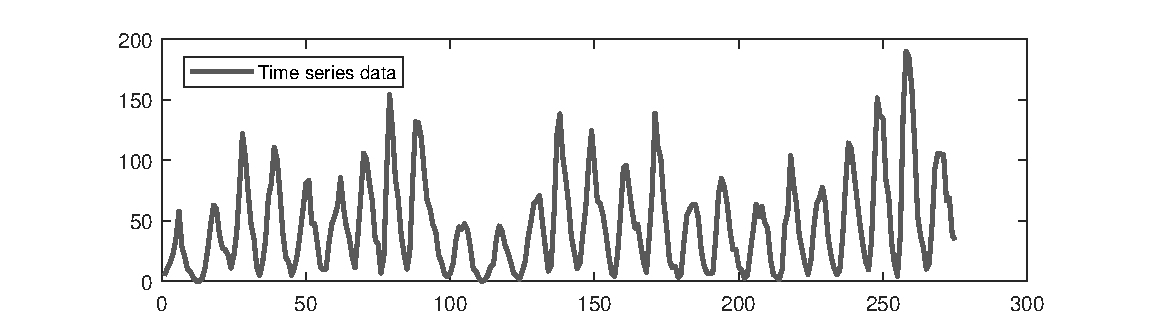
\includegraphics[scale=0.75, width=9cm]{figure3.eps}

\\
\begin{center}Figure 1. Time series data points\end{center}

\subsection{Training Data}
Considering the use of available data for its generalization in future prediction, we have used the Bayesian regulation backpropagation algorithm as it gave best results compared to Levenberg-Marquardt backpropagation. In the matlab environment we used the fitnet network with two hidden layers with 10 neurons in the first hidden layer and 5 neurons in the second hidden layer. The fitnet network uses Hyperbolic Tangent function on the hidden layers and a linear function on the output layer. This allows the neural network to adapt to the time series data. Additionally 5\% of the Data vectors were randomly pulled out to use as validation data leaving the other 95\% for training. Early stopping was used with the validation data with a failure number of 50 iterations before the early stopping was executed.\\

Bayesian regulation backpropagation is a method of training with automated regularization. This should help to prevent overfitting and increase the generalization. When finished training it was found that our network has an effective number of parameters of 103 out of 170. Since it converged to this number over about 50 iterations it is understood that this is a good indicator that the network is not overfitting. 

\subsection{Testing Data}
While training during the early stages of this project, it was observed that the random initialization to the order of the data and which data was chosen as validation data dramatically affected how well the network was able to learn and generalize. It was determined that since both the size of the network and the amount of given data are so small, minor changes to the random order of the data have a large impact. To solve this problem the network after training was finished the network was tested against the last 30 data points using the same method as the final prediction in order to predict the last 30 data points. This method allows us to actually compare the prediction of the neural network against real data to see how it will actually perform. The training and testing were done repeatedly in order to find the seeded network that produces the lowest MSE when comparing the prediction to the actual data. Once a sufficiently accurate and generalized prediction was obtained the final prediction was created. An example of this method can be seen in figure 2. below. \\

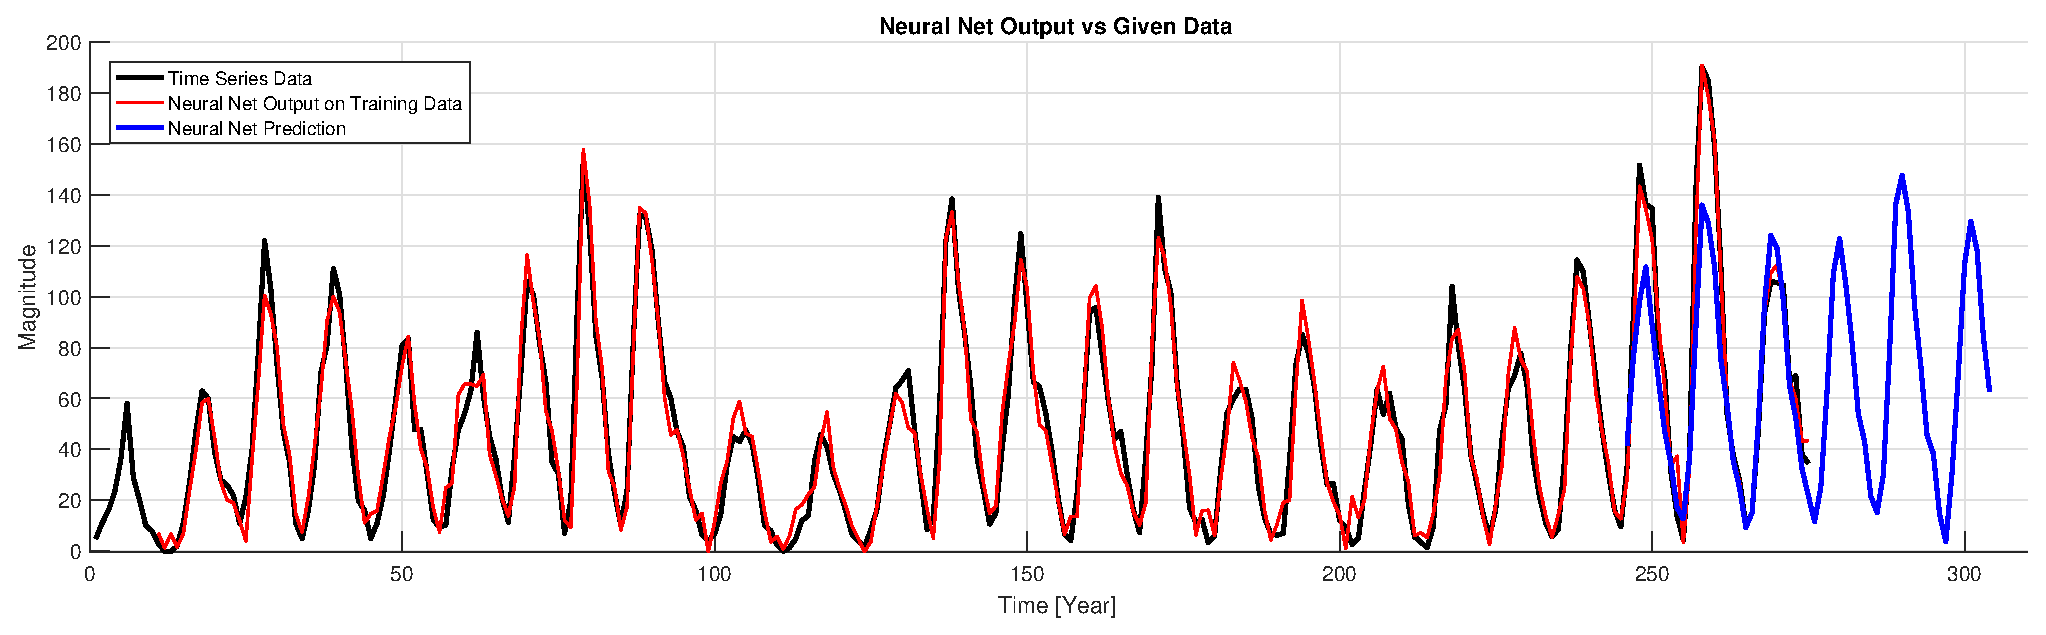
\includegraphics[scale=0.6, width=8cm]{figure2.eps}

\\
\begin{center}Figure 2. Neural Network prediction of the training data outputs\end{center}\\

\section{Results & Discussion}

The neural network was trained and the tested data had a mean square error of 682.2546. As mentioned above, the errors could still be reduced but the reduced error might not generalize the function. This is the trade off that has to be made in time series predictions because of the uncertainty in the functions. Adding to this fact, the time series data given in this problem is not monotonic which makes this even more difficult for any training algorithm to achieve global minimum that reduces the cost function.\\

Further, more intense machinery for this problem like reinforcement learning methods for time series prediction could yield better results. Figure 3. below shows the prediction of the neural network for the next 30 points.\\

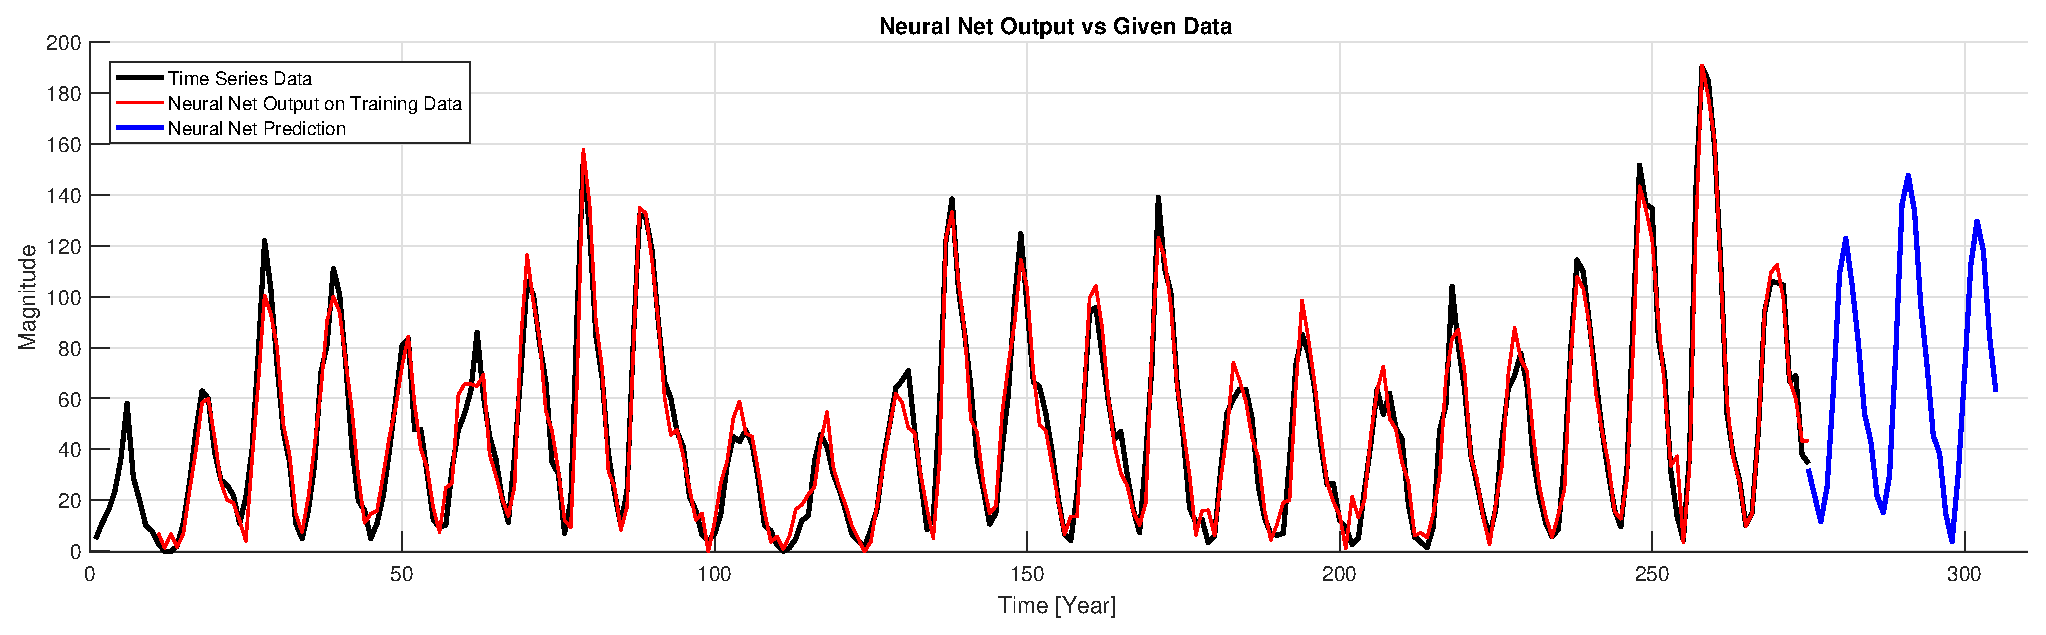
\includegraphics[scale=0.6, width=8cm]{figure1.eps}

\\
\begin{center}Figure 3. Neural Network prediction of the next 30 points\end{center}

\section{Conclusion}
Considering analysis made by our team for the given problem, prediction of time series data set based on the given data set is highly dependent on the quantity of data. Since our method tries to generalize the output function based on minimum data set, and also there is no monotonic behavior associated with the data makes it highly difficult to solve this problem. Therefore the bottom line is even if we build a neural network with near zero mean square error, there is no guaranty that the prediction function might predict it with near certainty. But the prediction could definitely be improved with more amount of data and features which might give the neural network an extra edge to predict the future data better.

\begin{thebibliography}{3}

\justifying

\bibitem{}
{Gianluca Bontempi. (2013). Machine Learning Strategies for Time Series Prediction} - 
\url{http://www.ulb.ac.be/di/map/gbonte/ftp/time_ser.pdf}
 
\bibitem{}
{Mathworks.com 'Levenberg-Marquardt Algorithm' [Online].}
\url{Available: https://www.mathworks.com/help/nnet/ref/trainlm.html}

\bibitem{}
{Mathworks.com 'Bayesian Regularization Algorithm' [Online].}
\url{Available:  https://www.mathworks.com/help/nnet/ref/trainbr.html}

\end{thebibliography}

\begin{IEEEbiography}

% /[{\includegraphics[width=1in,height=1.25in,clip,keepaspectratio]{picture}}]{John Doe}

\end{IEEEbiography}





\end{document}

